\section{Introduction}
\label{introduction}
VTK is an open source cross-platform software system used for scientific data
processing, analysis, and visualization. It was originally developed to
supplement a textbook on object-oriented computer graphics
programming~\citep{schroeder_visualization_2006, geveci_vtk_2012}.  VTK has a long history of volume rendering and, unfortunately, that
history was evident in its large collection of classes used to render volumes.
While these methods were state-of-the-art at the time they were implemented,
given VTK's 20+ year history, many of these methods are now obsolete. Recently,
there has been a major effort~\citep{hanwell_visualization_2015} undertaken to
re-write VTK's rendering backend, which was based on a now-deprecated legacy 
OpenGL API, to one based on a modern, programmable-pipeline OpenGL
API~\citep{shreiner_opengl_2013}. 

This new rendering subsystem was designed to
support the latest technological advances in the graphics hardware industry.
We aimed to consolidate the large number of
volume mappers into two: one supporting accelerated rendering using the Graphics
Processing Unit (GPU) and a second, parallel implementation on the Central
Processing Unit (CPU). In addition, a~\texttt{vtkSmartVolumeMapper} class was
added to assist application developers in providing an automatic run-time selection of
the appropriate volume rendering techniques based on system configuration
(see~\Autoref{fig:inheritancegraph}).

\begin{figure}
  \centering
  \begin{subfigure}[b]{\columnwidth}
    \centering
    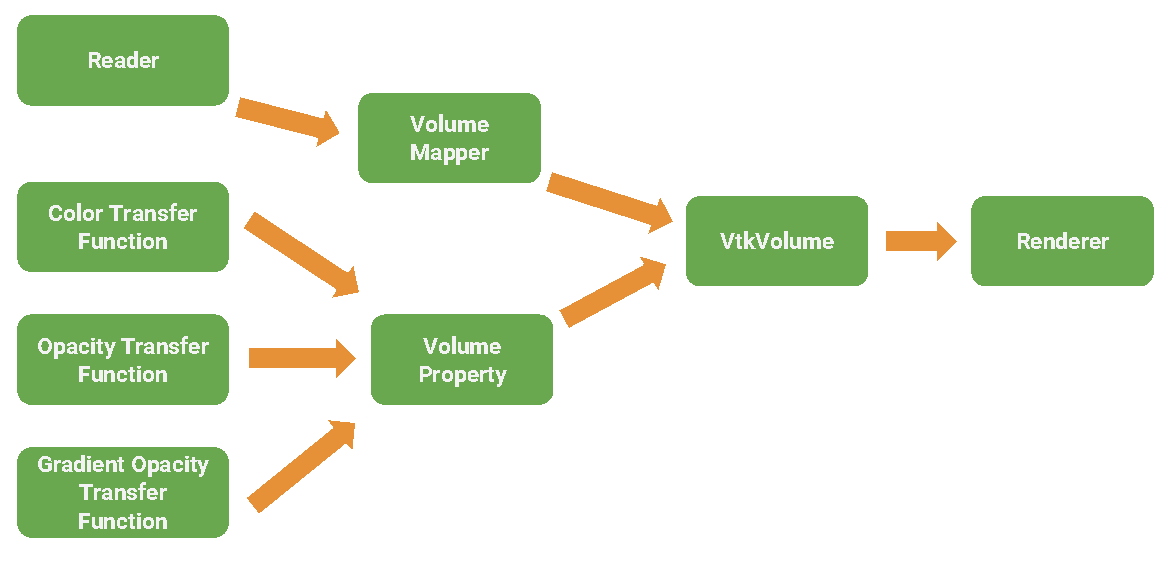
\includegraphics[width=\columnwidth, height=0.4\textheight]{vtk_volume_pipeline}
    \caption{VTK pipeline for volume rendering which is similar to the polygonal
      rendering pipeline in VTK}
    \label{fig:pipeline}
  \end{subfigure}\vfill
  \begin{subfigure}[b]{\columnwidth}
    \centering
    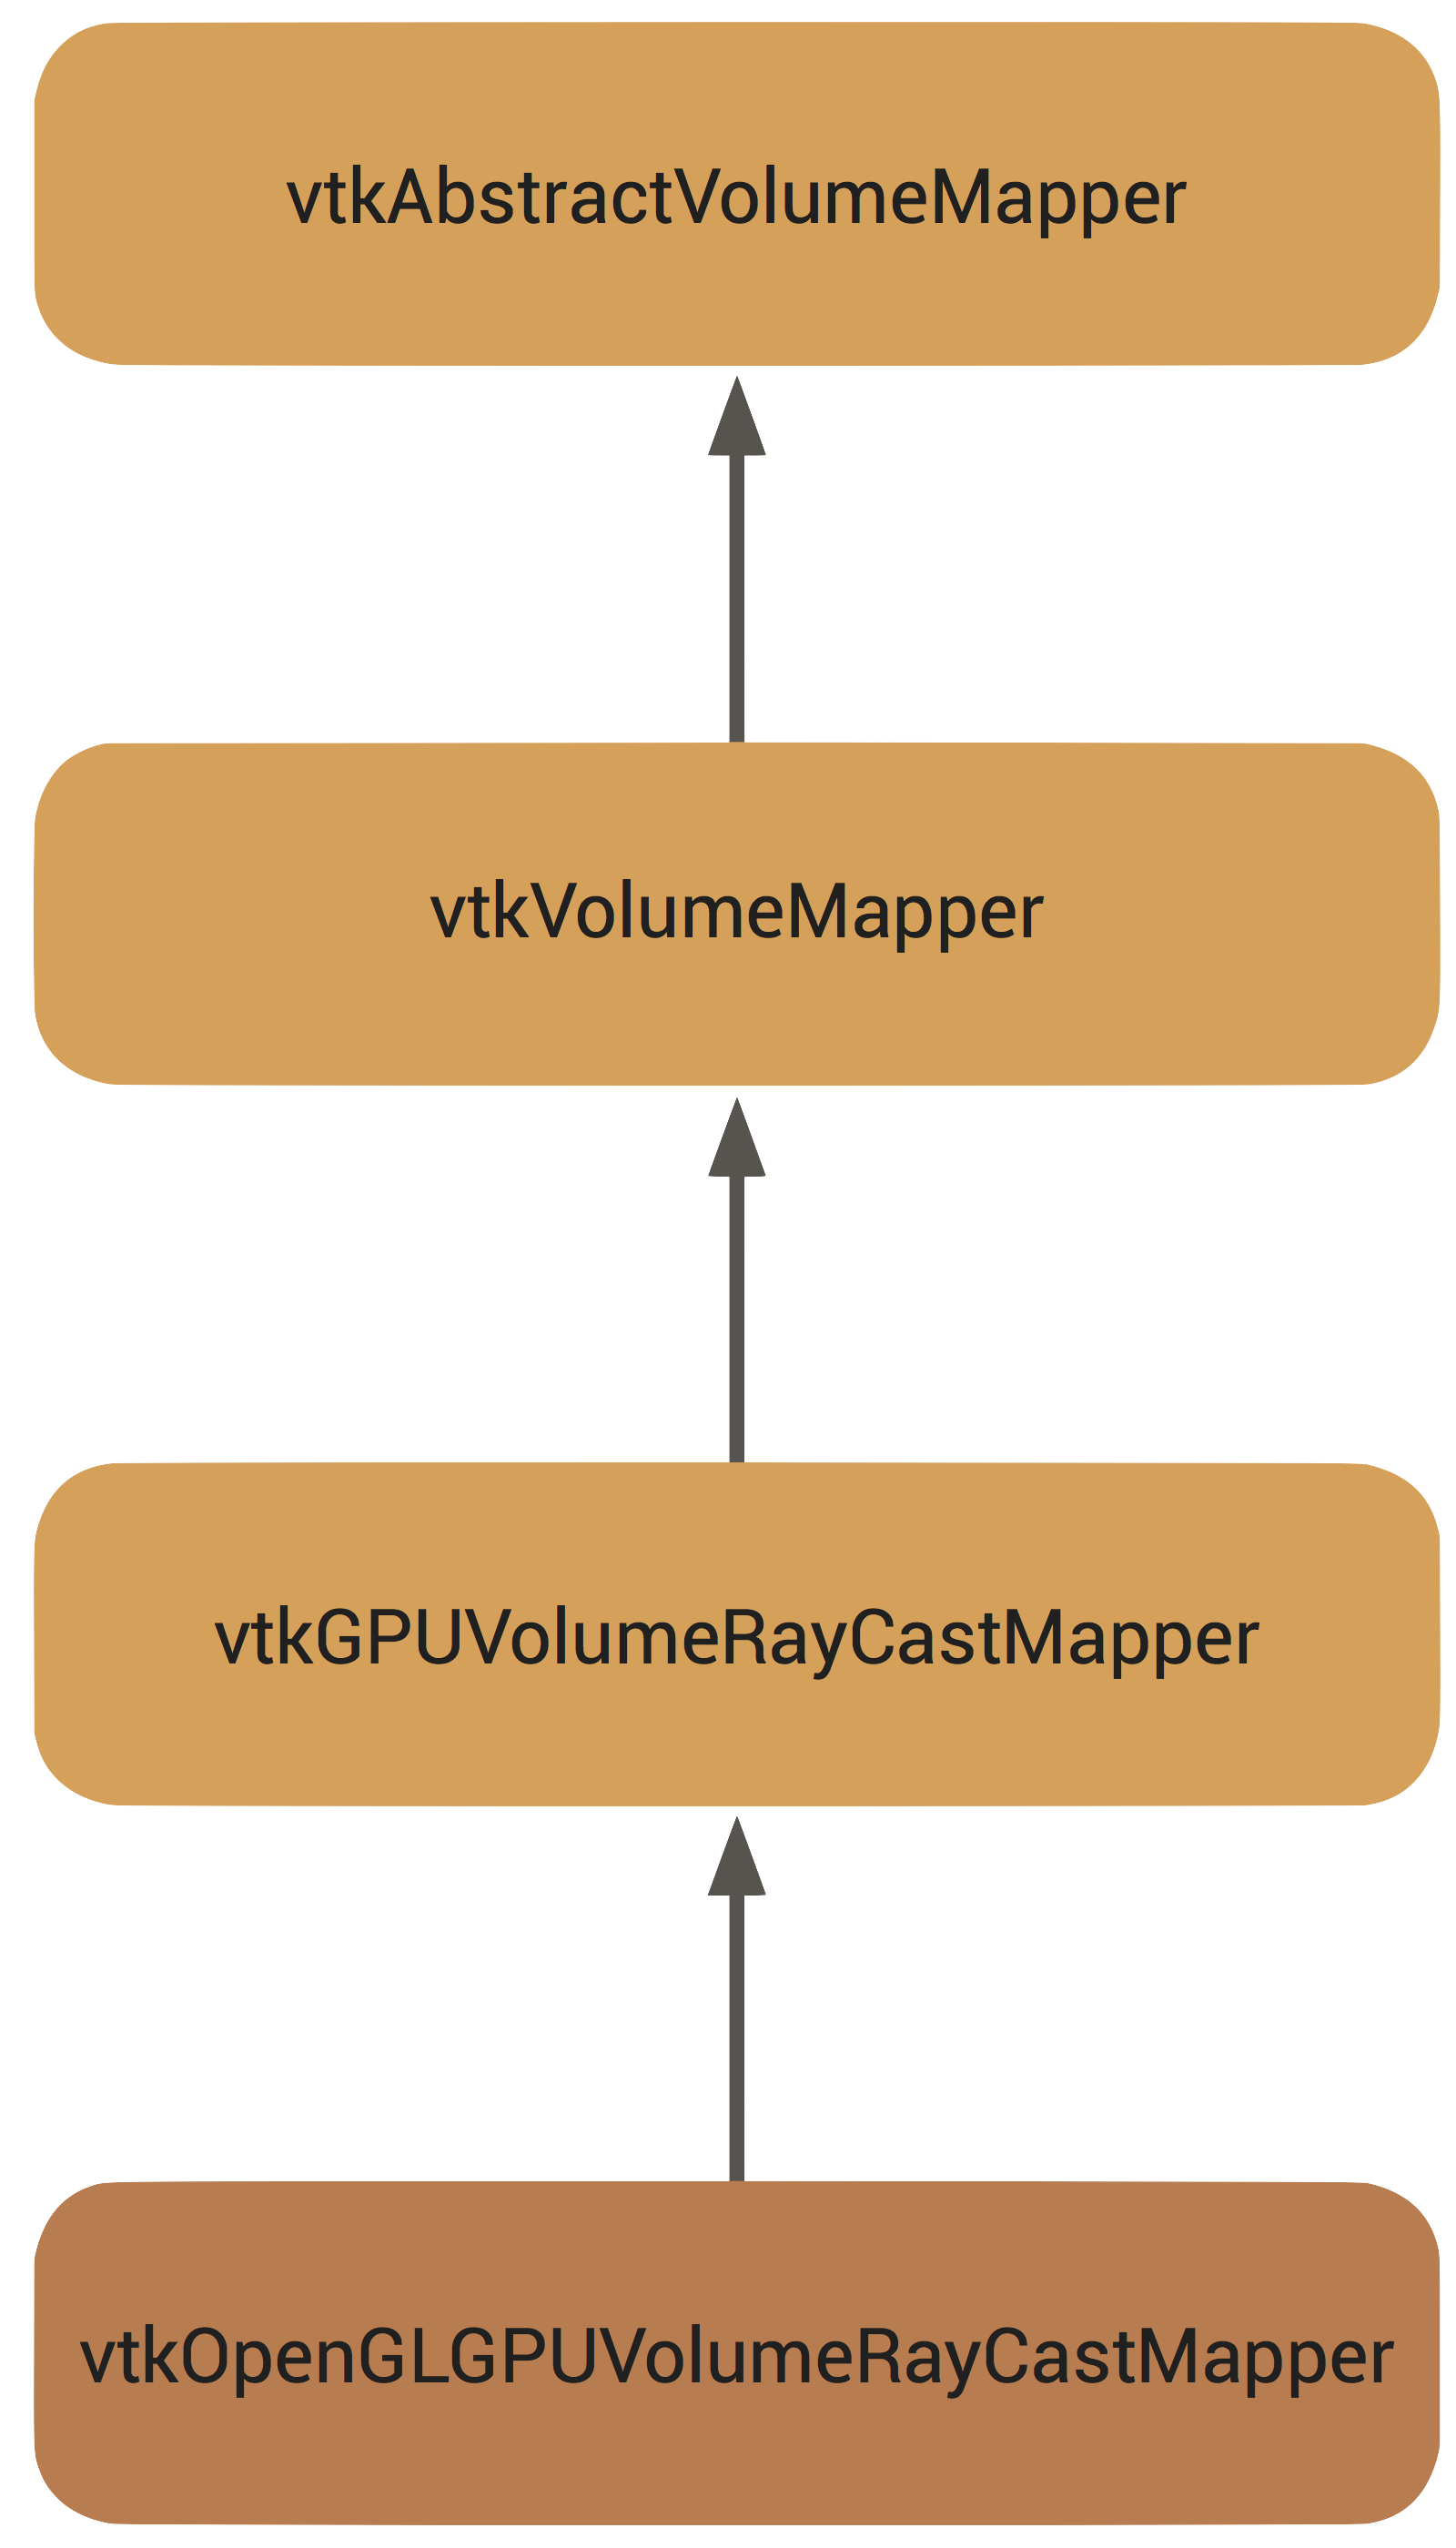
\includegraphics[width=\columnwidth, height=0.4\textheight]{inheritancegraph}
    \caption{Graph depicting C++ class hierarchy for
      the various volume mappers in VTK}
    \label{fig:inheritancegraph}
  \end{subfigure}
  \caption{Volume rendering works within the constructs of the VTK pipeline
    mechanism}
  \label{fig:pipeline-inheritancegraph}
\end{figure}

Thus, a primary objective of this OpenGL modernization effort was the
subject of this article: to create a cross-platform, multi-functional,
high-performance volume renderer supporting both serial and parallel execution
modes capable of supporting such complex applications as
ParaView~\citep{ahrens_paraview:_2005,ayachit_paraview_2015} or 3D
Slicer~\citep{fedorov_3d_2012}.  While volume rendering using ray-casting
approach is currently the state-of-the-art, the strength of our work is the
conglomeration of many principles of the chosen technique, which has resulted in a
fast-performing, pipeline-based volume render that works for multiple types and
formats of the scientific and medical datasets. 

The goal of our effort is as follows:

\begin{itemize}
  \item Enable ubiquitous, cross-platform, high-performance support for volume
    rendering across all major operating systems and computing environments
    (desktop, VR, mobile).

  \item Ensure that the new volume visualization subsystem provides support for
    VTK-based pipeline and data-flow networks, thereby providing a flexible
    system addressing a wide variety of scientific and medical data
    visualization use-cases.

  \item Provide a variety of useful features at interactive frame rates such as
    clipping, cropping, gradient opacity, mixed geometry-volume translucent
    rendering, and on-demand shader composition.
\end{itemize}

We created a replacement for the OpenGL fixed function pipeline
based~\texttt{vtkGPUVolumeRayCastMapper}. The new mapper, which shares the same
name but uses a modern OpenGL programmable pipeline, can be used
via~\texttt{vtkSmartVolumeMapper} or instantiated directly. The new mapper with
its OpenGL-VTK implementation improves the management of textures in the mapper,
and benefits both geometry and volume rendering by sharing common code between
them. 

While volume ray-casting itself is
a well-known technique, developing a volume renderer that works with variety of
data formats and types, supports many essential features for medical and
scientific computing, works across all major computing platforms, and performs
well at interactive frame rates with very large datasets was a challenging task. 
Our team met this challenge with an in-depth knowledge of the data, graphics pipeline, the VTK framework, and user requirements.  

In the next section, we describe the
technical details behind the effort to produce the resulting modern,
cross-platform volume renderer delivered to the open source VTK community.
